\subsection{Itération n°3}

\subsubsection{Configuration, modifications et résultats attendus}

Nous redimensionnons la récompense à nouveau de sorte à ce que la récompense sur un épisode soit compris entre $0$ et $100$. En faisant cela, nous souhaitons réduire l'amplitude de la récompense et avec le bruit associé. En réduisant le bruit, le gradient converge plus facilement vers un minimum.

Pour borner la récompense sur un épisode entre $0$ et $100$, nous divisons l'équation~\ref{eq:itr2_rescale} par le nombre de pas par épisode soit $200$.

Nous attendons à avoir une récompense par épisode bornée par $0$ et par $100$. Par la réduction d'échelle, nous attendons à obtenir une courbe moins bruitée et croissante. En effet, la réduction du bruit permet une variation plus fine est poids et des biais.  Donc d'avoir une évolution plus douce. Celle-ci permet de converger vers un minimum ce qui améliore la politique et par conséquent la récompense.

\subsubsection{Analyse}

\begin{figure}[H]
    \centering
    \begin{subfigure}{0.3\textwidth}
        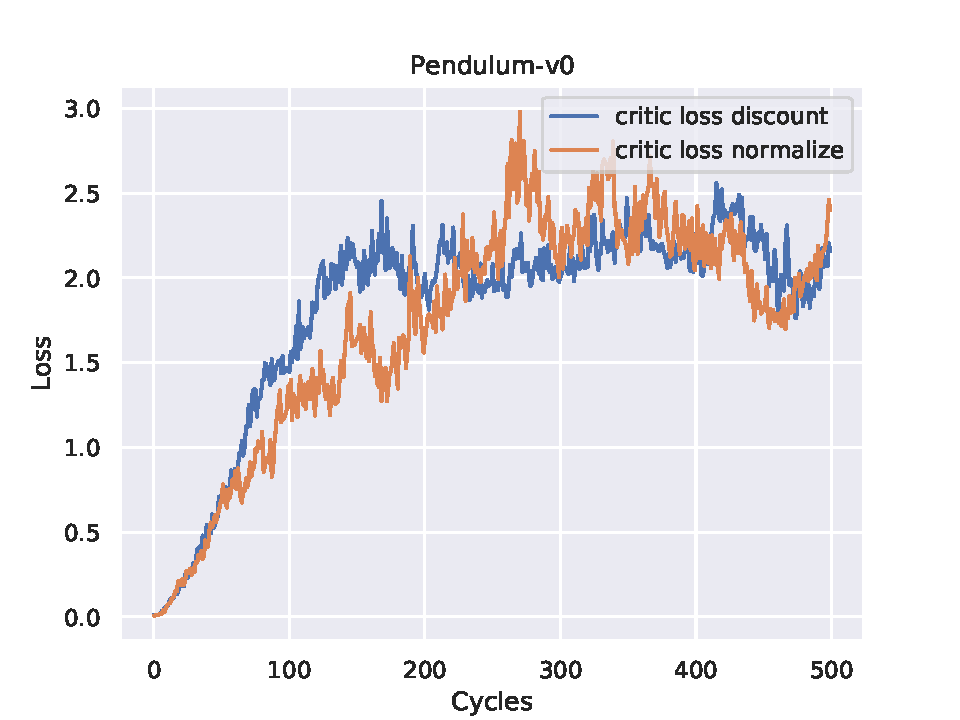
\includegraphics[width=\textwidth]{figures/iteration3/critic_loss_Pendulum-v0_pg_dataset_td_eval_True_cycles_500_trajs_20_batches_20_gamma_0.99_nstep_5_l.pdf}
        \caption{Fonction de perte de la critique}
    \end{subfigure}
    \begin{subfigure}{0.3\textwidth}
        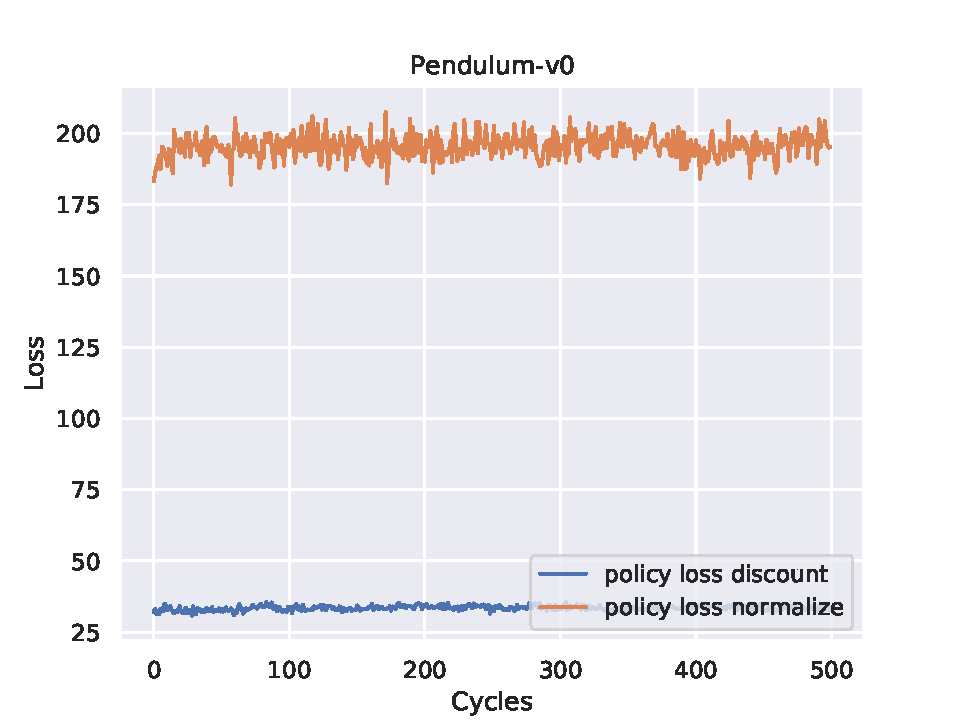
\includegraphics[width=\textwidth]{figures/iteration3/policy_loss_Pendulum-v0_pg_dataset_td_eval_True_cycles_500_trajs_20_batches_20_gamma_0.99_nstep_5_l.pdf}
        \caption{Fonction de perte de la politique}
    \end{subfigure}
    \begin{subfigure}{0.3\textwidth}
        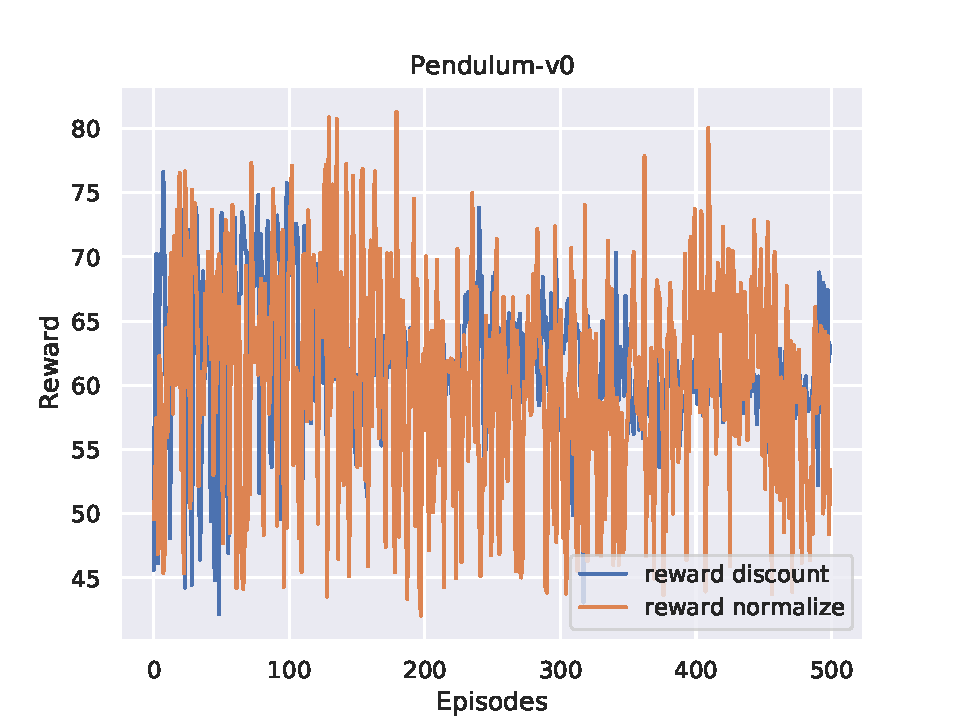
\includegraphics[width=\textwidth]{figures/iteration3/rewards_Pendulum-v0_pg_dataset_td_eval_True_cycles_500_trajs_20_batches_20_gamma_0.99_nstep_5_lr_ac.pdf}
        \caption{Récompenses des épisodes}
    \end{subfigure}
    \caption{Résultats obtenus pour la critique, la politique et la récompense}
    \label{fig:itr3_results}
\end{figure}

Nous observons que notre récompense est bien bornée entre 0 et 100 mais ne croît pas comme espéré. La récompense obtenue par la méthode \emph{discount} semble même se stabiliser aux alentours de 60.

Nous observons que la fonction de perte de la politique est relativement constante. Ce résultat est tout à fait singulier. Nous en déduisons qu'il y a un problème dans l'apprentissage de la politique. Malheureusement, nous ne somme pas parvenu à identifier le problème

Comme précédemment, la fonction de perte de la critique ne décroît toujours pas.

\begin{figure}[H]
    \centering
    \begin{subfigure}{0.3\textwidth}
        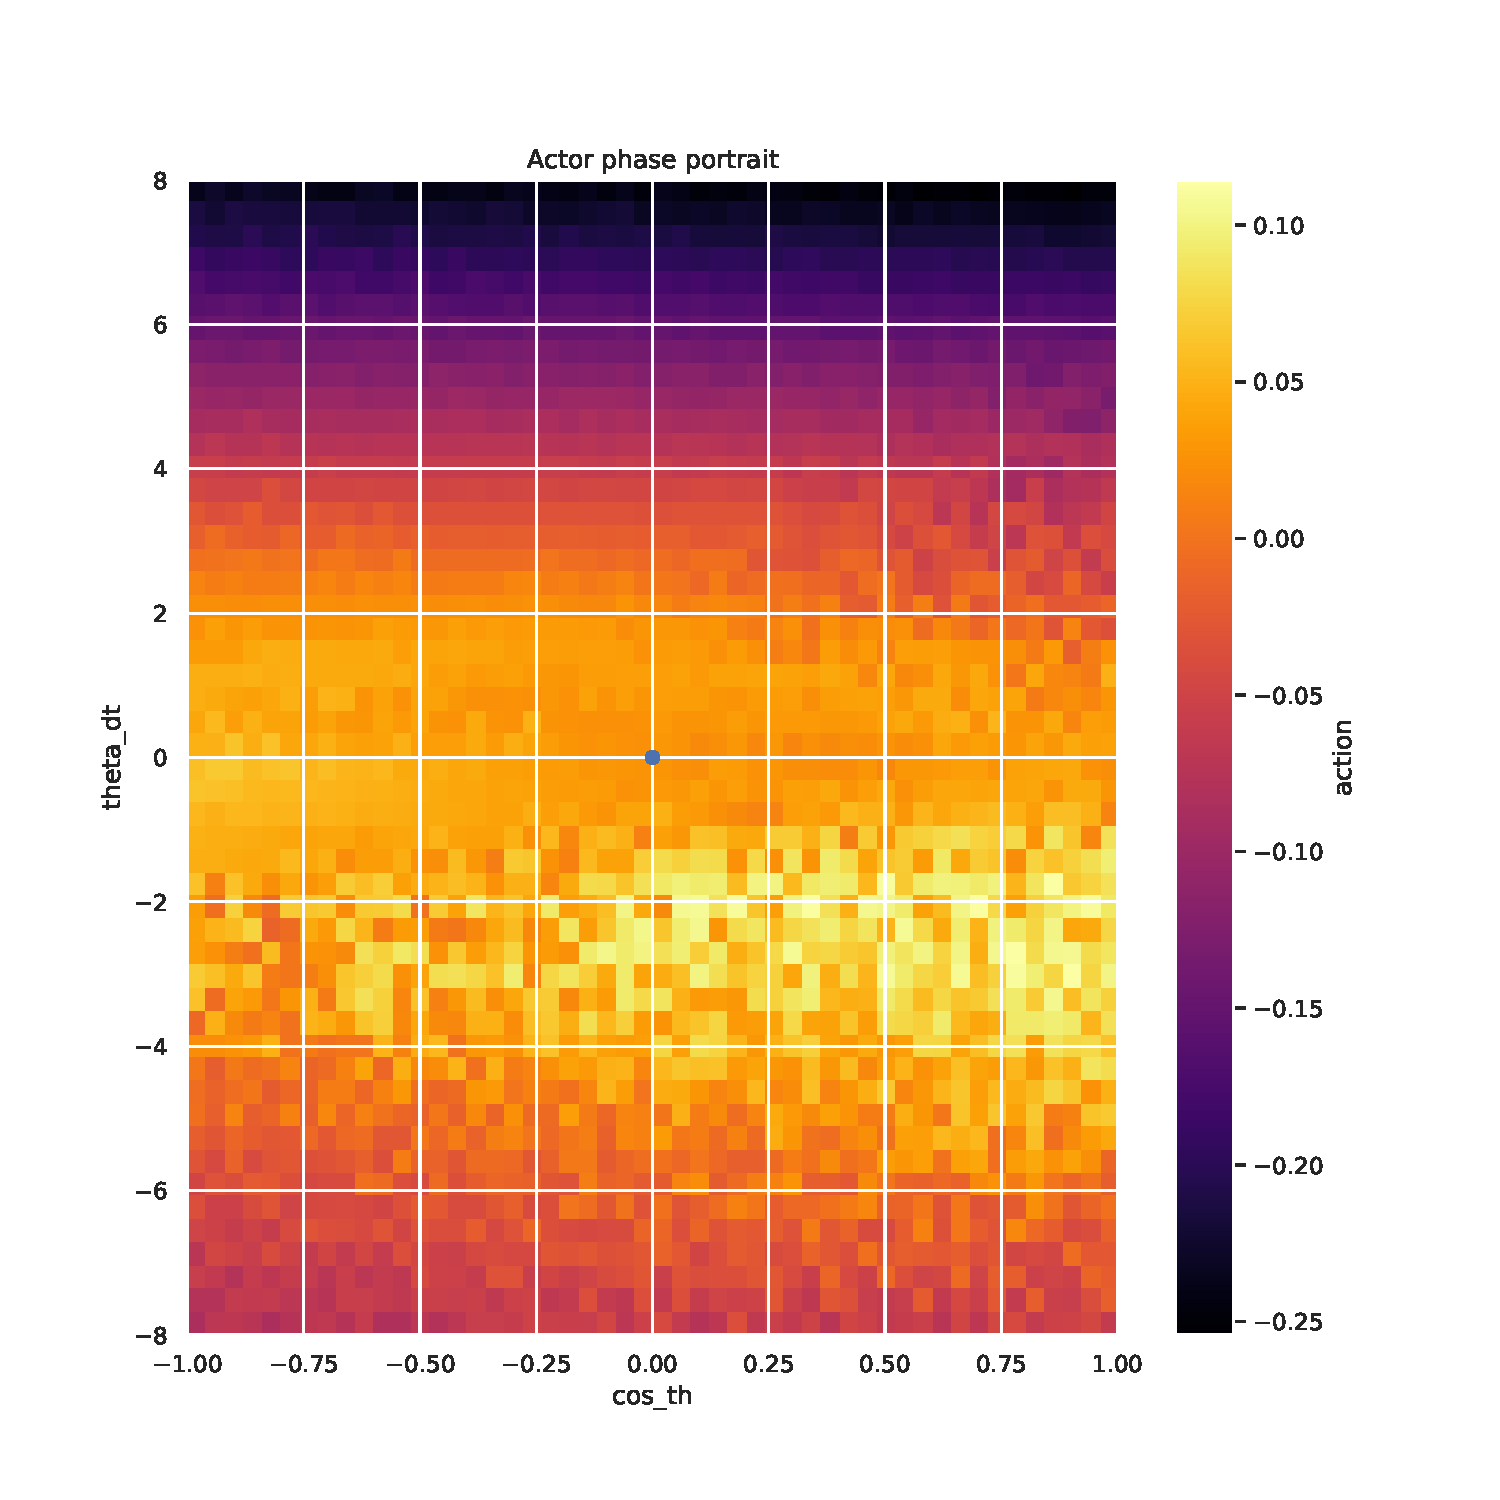
\includegraphics[width=\textwidth]{figures/iteration3/0_actor_discount__ante_Pendulum-v0.pdf}
        \caption{Acteur naïf}
    \end{subfigure}
    \begin{subfigure}{0.3\textwidth}
        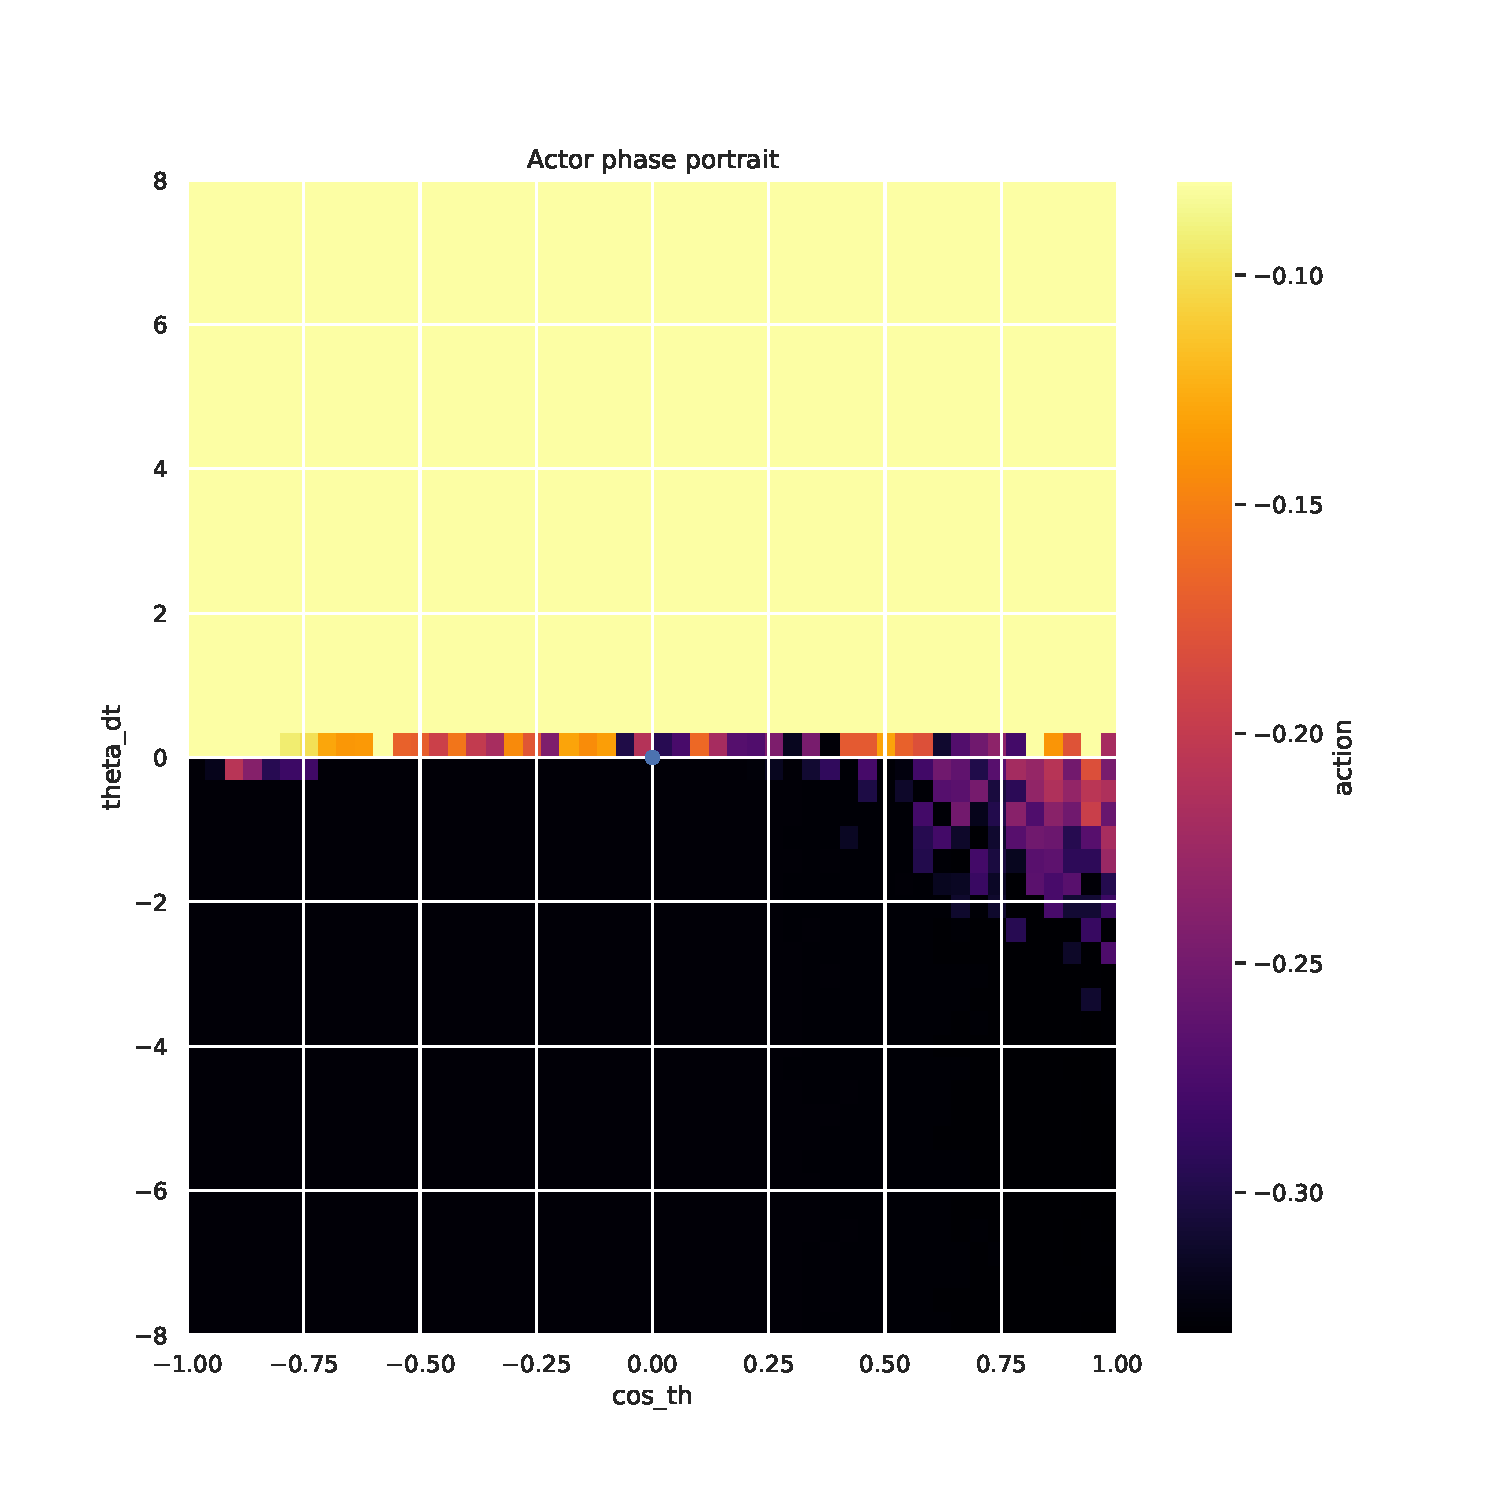
\includegraphics[width=\textwidth]{figures/iteration3/0_actor_discount__post_Pendulum-v0.pdf}
        \caption{Acteur entraîné}
    \end{subfigure}
    \begin{subfigure}{0.3\textwidth}
        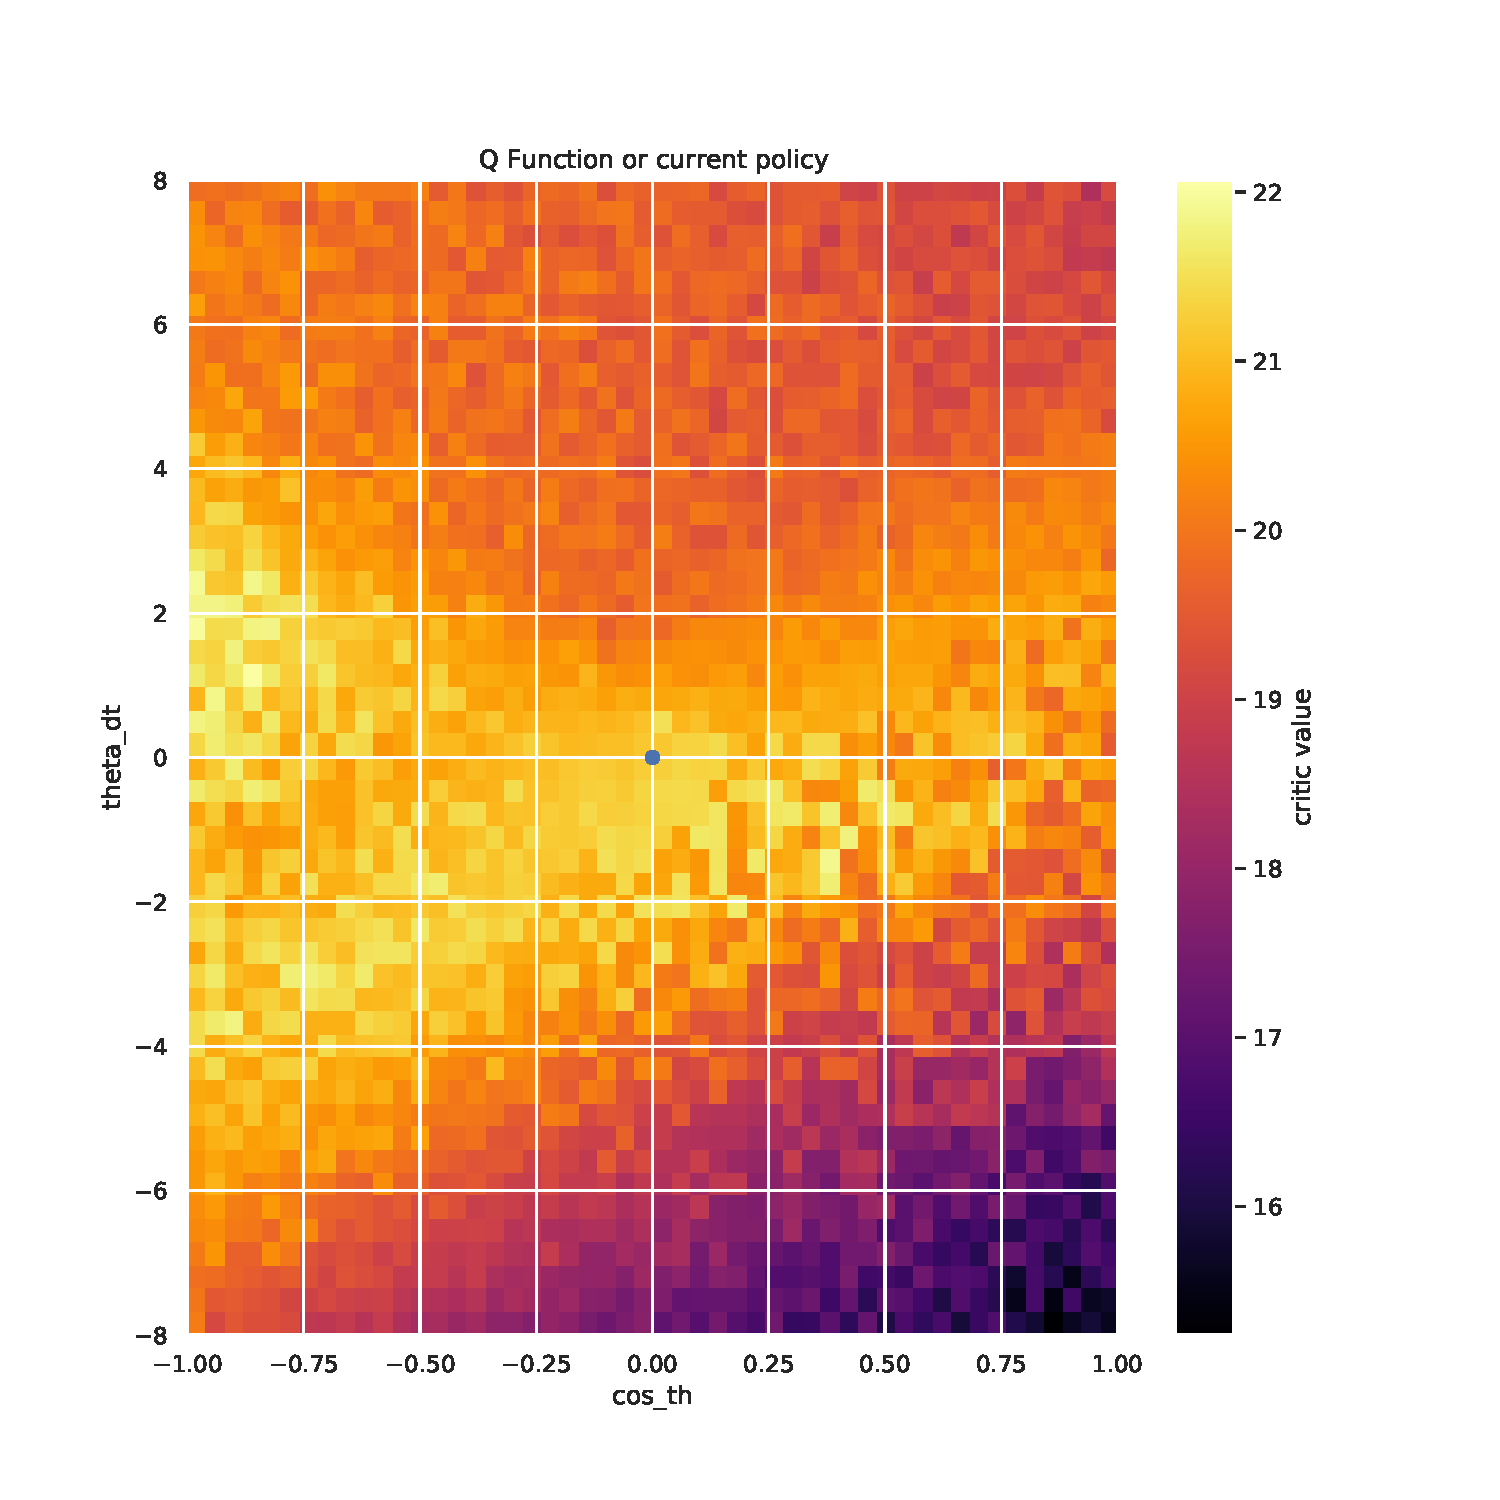
\includegraphics[width=\textwidth]{figures/iteration3/0_critic_discount_post_Pendulum-v0.pdf}
        \caption{Critique entraînée}
    \end{subfigure}
    \caption{Valeurs de l'acteur et de la critique avec la méthode discount pour le calcul de la récompense}
    \label{fig:itr3_discount}
\end{figure}

La plage d'action de l'acteur n'est pas cohérente avec ce que l'on attend. nous préférerions une plage d'action comprise entre $-2$ et $2$. L'apprentissage définitivement mauvais car où qu'il soit et peu importe sa vitesse, il continuera de tourner.

La critique n'est toujours pas intéressante au vu de ses zones de préférence sur l'ensemble de l'intervalle de $\cos(\theta)$. De plus, la critique semble aussi favoriser la position en bas du pendule avec une vitesse faible qui ne lui feras pas quitter cet été pourtant à éviter.

\begin{figure}[H]
    \centering
    \begin{subfigure}{0.3\textwidth}
        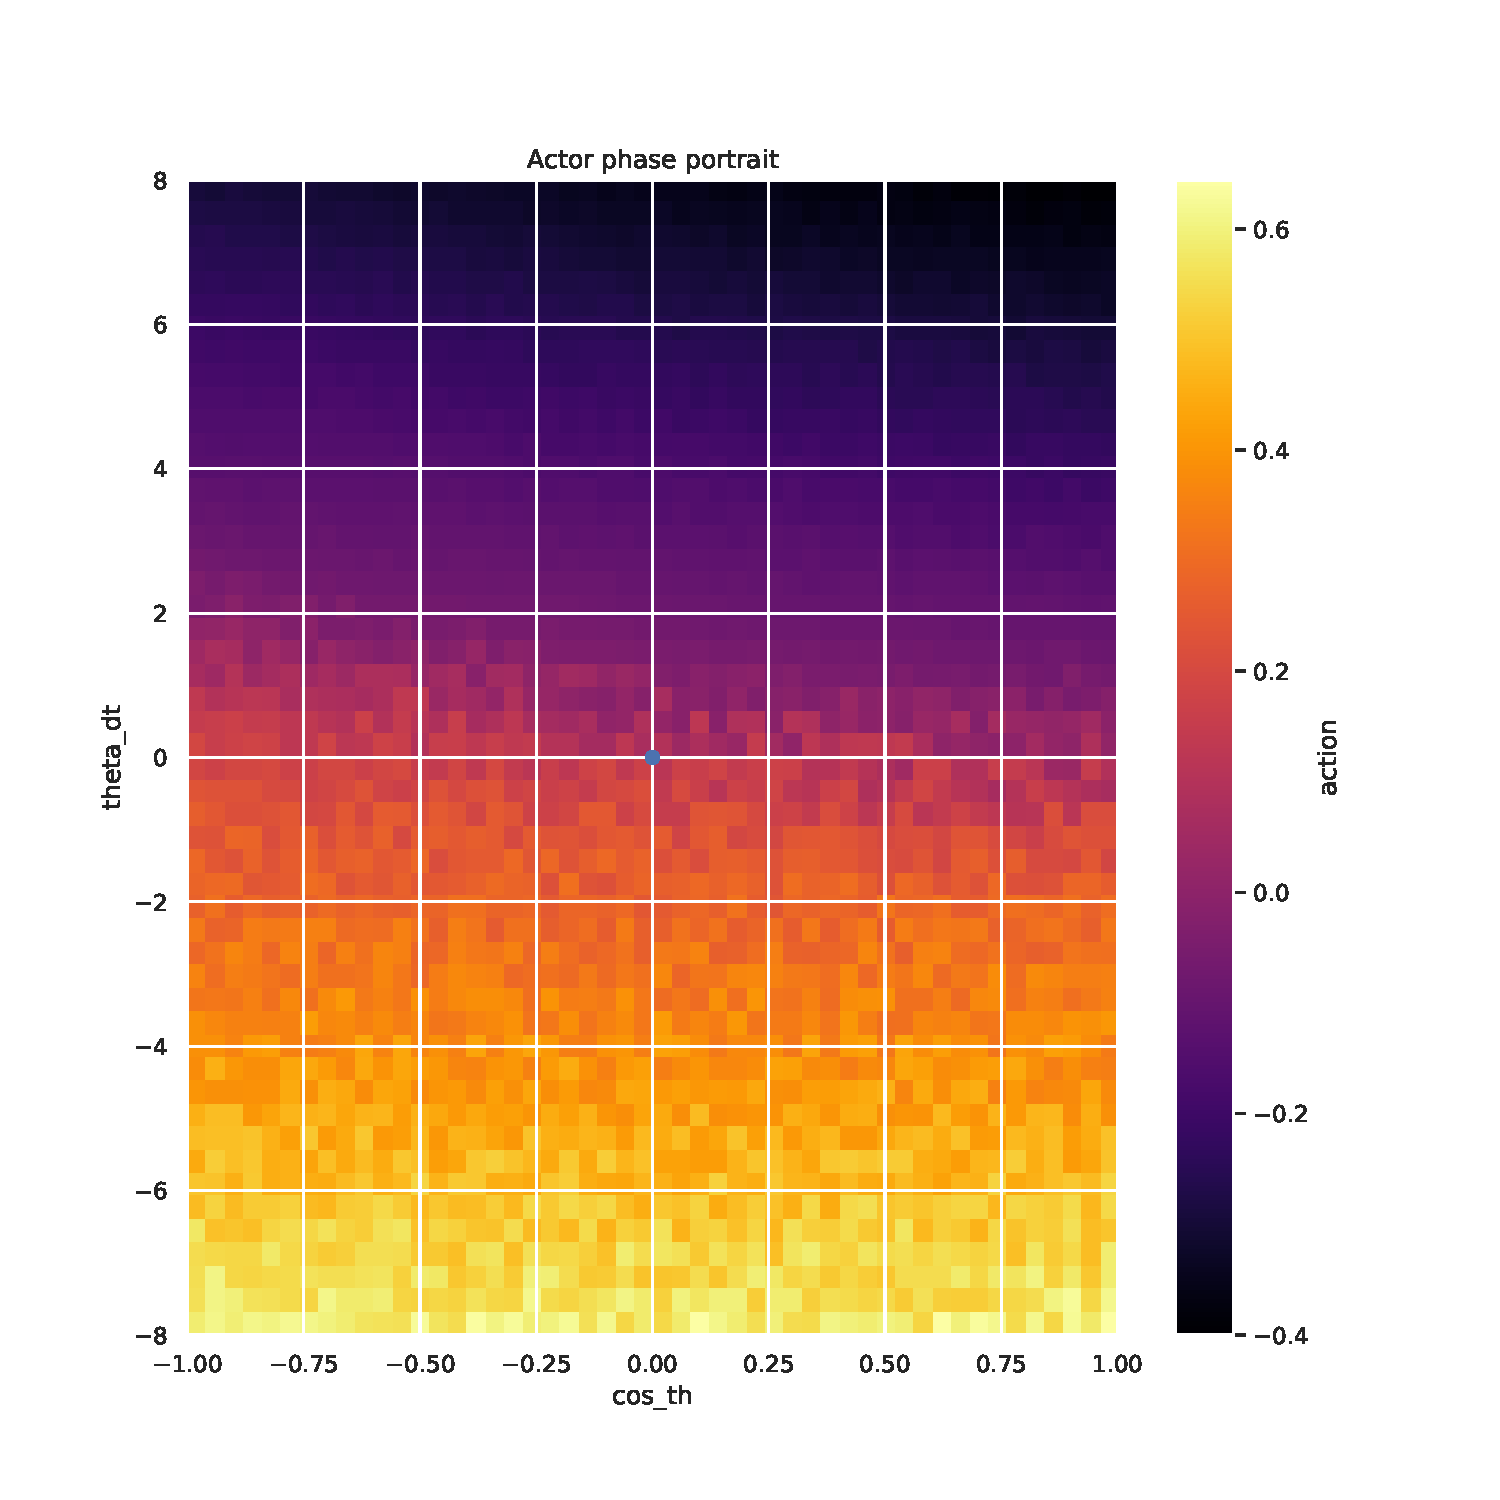
\includegraphics[width=\textwidth]{figures/iteration3/0_actor_normalize__ante_Pendulum-v0.pdf}
        \caption{Acteur naïf}
    \end{subfigure}
    \begin{subfigure}{0.3\textwidth}
        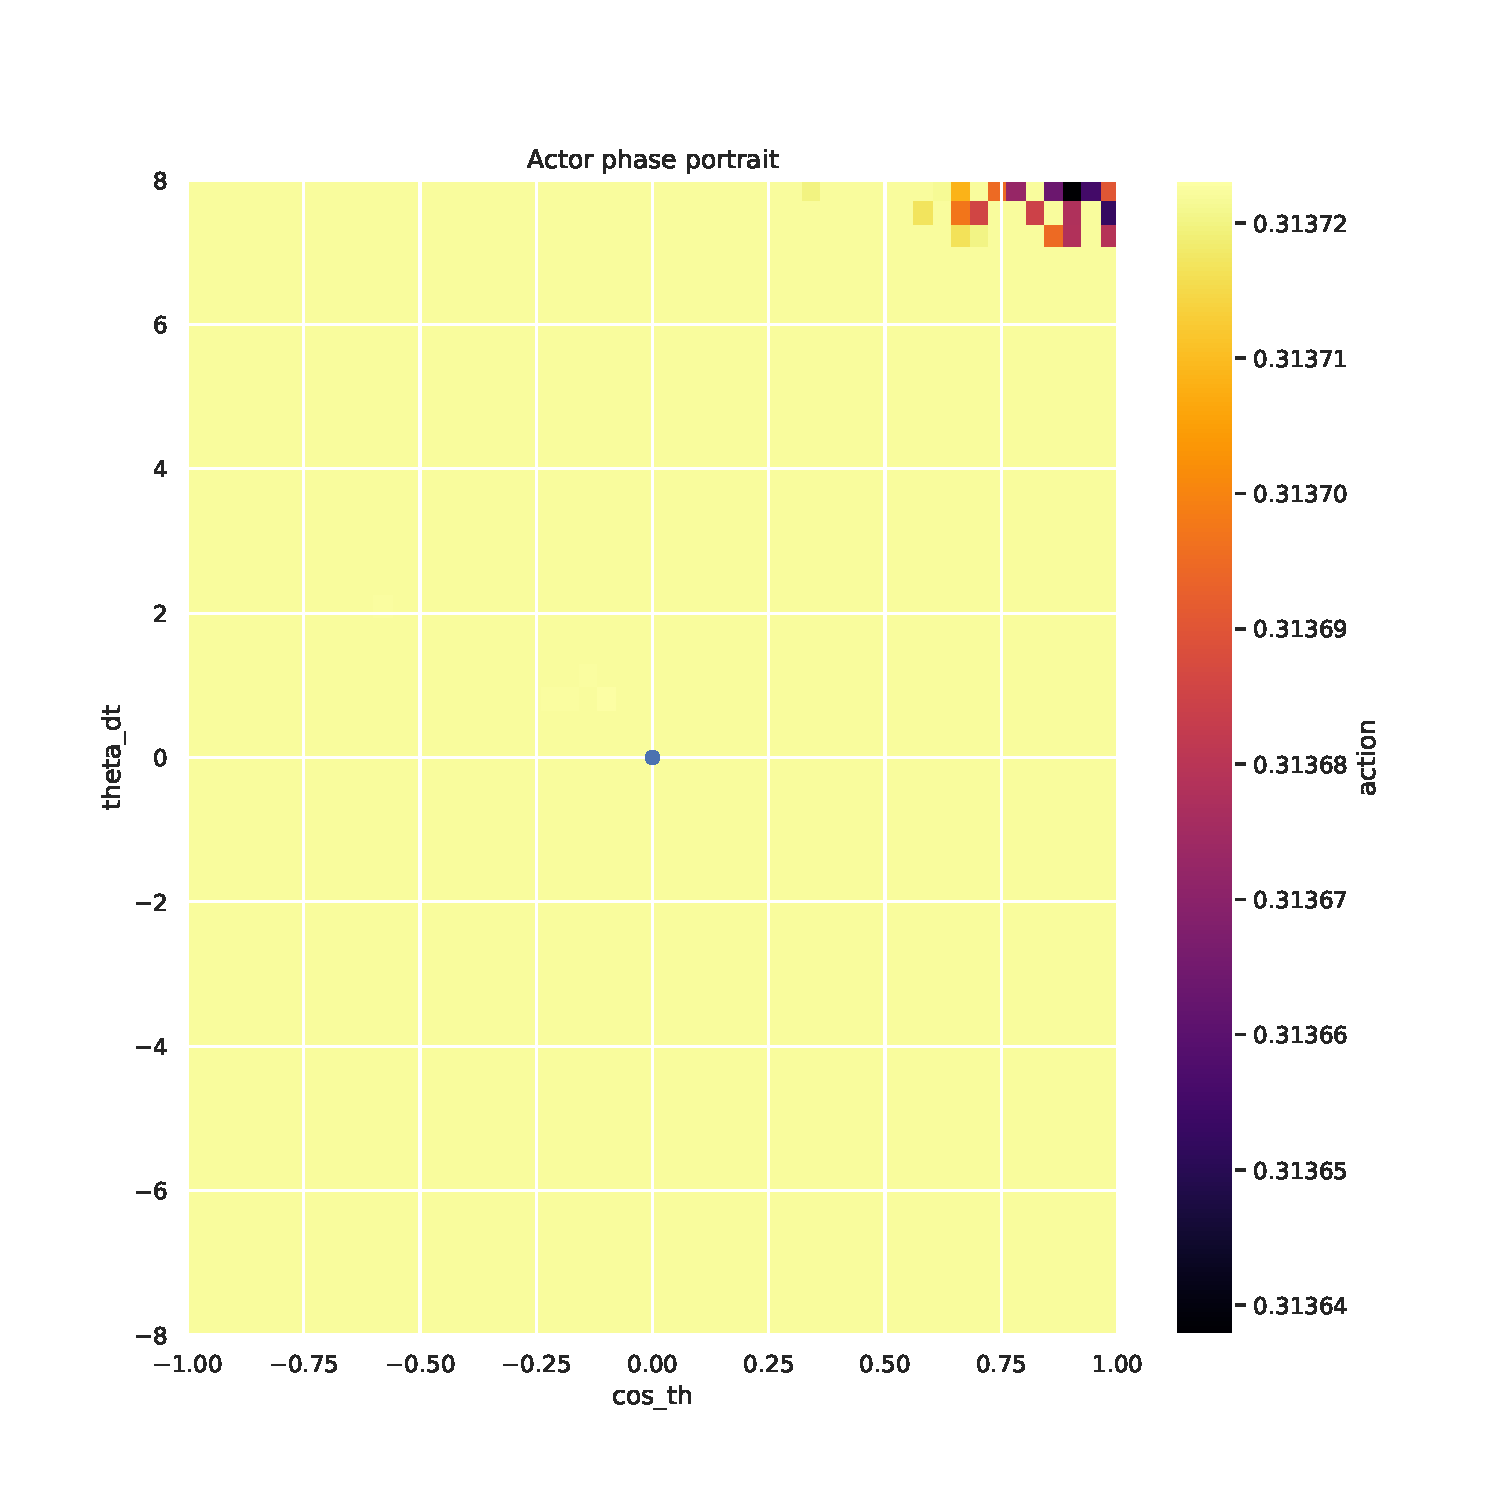
\includegraphics[width=\textwidth]{figures/iteration3/0_actor_normalize__post_Pendulum-v0.pdf}
        \caption{Acteur entraîné}
    \end{subfigure}
    \begin{subfigure}{0.3\textwidth}
        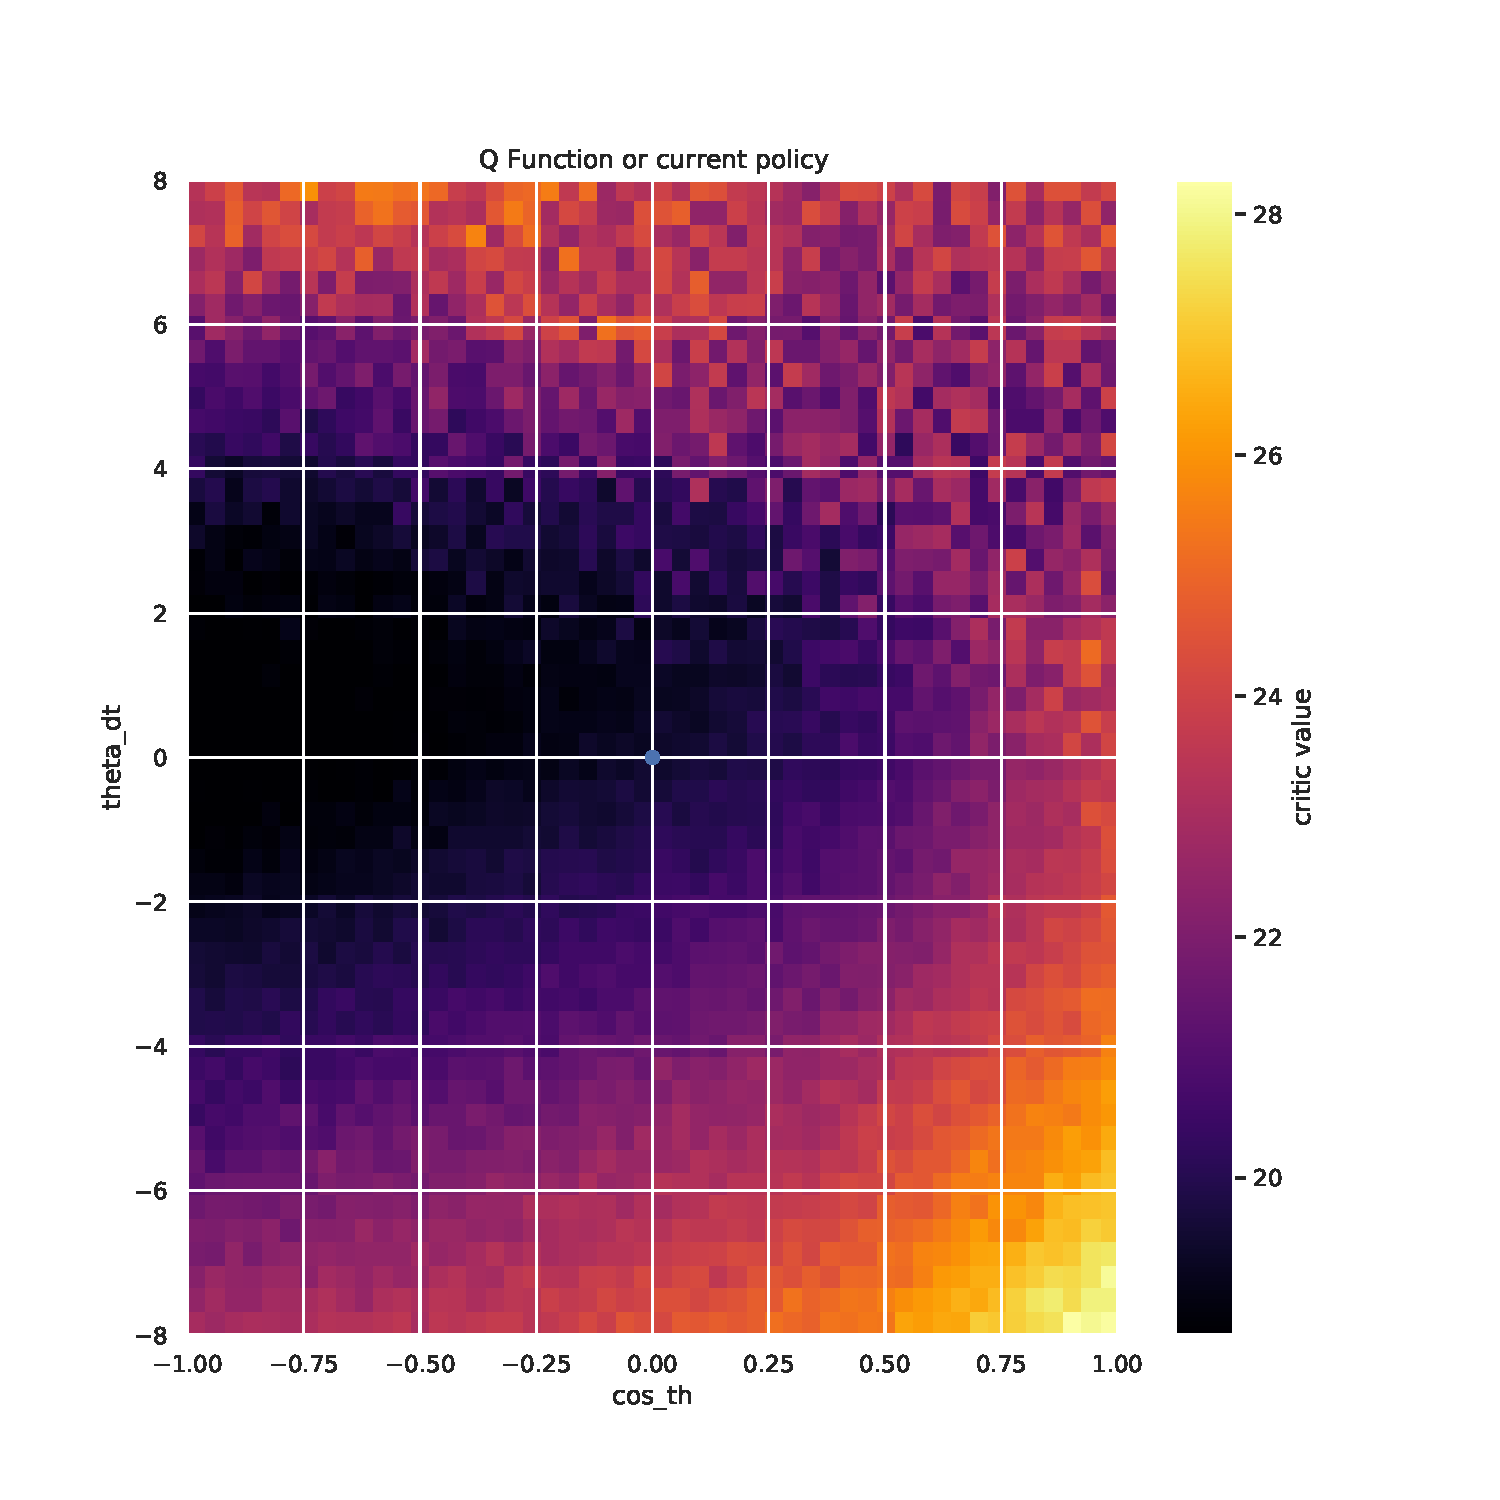
\includegraphics[width=\textwidth]{figures/iteration3/0_critic_normalize_post_Pendulum-v0.pdf}
        \caption{Critique entraînée}
    \end{subfigure}
    \caption{Valeurs de l'acteur et de la critique avec la méthode normalize pour le calcul de la récompense}
    \label{fig:itr3_normalize}
\end{figure}

La méthode \emph{normalize} ne présente toujours pas d'acteur entraîné correctement. Dans ce cas, la politique va faire tourner le pendule à la même vitesse et dans le même sens peu importe son état.

La critique, quant à elle, semble bien défavoriser le fait d'être en bas du pendule mais préfère être à grande vitesse une fois en haut. Cela n'est donc toujours pas ce que l'on attend.